\chapter{Preliminaries}
\label{chap:num_1}

The chapter is going to provide the introduction to the core concepts of \textit{Semantic Web}, \solid{} and \lpa{} platform. As the concepts explained here will be often referred to in further chapters, it is important to get familiar with them for a complete understanding of every consecutive chapter. 

\section{Semantic Web}
\label{sssec:semantic_web_intro}

The Semantic Web represents the next significant iteration in connecting data and information over World Wide Web. It adds an ability for a data to be linked from any source to any other source allowing computers to understand the semantics of it and perform increasingly complex computational operation on them. The major idea that makes Semantic Web technology and other data related technologies such as relational databases, is that it focused on preserving the meaning of the data rather than structuring it in efficient manner. 

There are three main technical specifications defining the Semantic Web technologies:
\begin{itemize}
	\item \gls{RDF}, is a data modelling language designed for Semantic Web. Every information in Semantic Web is represented in the RDF.
	\item \gls{SPARQL}, is a query language for Semantic Web. It is mainly designed for querying data across different data sets represented in RDF.
	\item \gls{OWL}, is a knowledge representation language for Semantic Web. It allows defining entities and concepts in a way that allows high reusability for many different applications and purposes.
\end{itemize}  

In other words, the usage of the technology stack mentioned above is what defines a Semantic Web application and differentiates it from any other technologies related to data.

\subsection{RDF}

The Resource Description Framework is a language for representing resources in World Wide Web (RDF Primer \cite{Miller:04:RP}). Every element of information in RDF is expressed as relation between entities. The entity in RDF is usually referred to as \textit{resource} and identified by \gls{URI}, in other terms anything identified by URI is a resource. The relation itself is expressed using \textit{triple} notation. A \textit{triple} notation is a statement written as follows, \texttt{\textbf{subject} \textbf{predicate} \textbf{object}}.

Consider the following example on listing \autoref{lst:intro_triple_example}. A \textit{subject} is a person identified by a URI, a \textit{predicate} identified by a URI describes the kind of relationship and lastly the \textit{object} is a resource similar to \textit{subject} and identified by a URI. In other words, the example demonstrating a sentence \textit{Person A knows Person B} expressed in RDF triple notation. A typical RDF document consists of many triple statements, together they can be represented as a directed \textit{graph}, where relation is presented as a directed edge between two vertices. The term graph will be often referred in \autoref{chap:num_4}  and \autoref{chap:num_5}.
 
\begin{listing}[ht]    
\begin{minted}[breaklines,frame=single,framerule=1pt]{text}
http://example.name#Altynbek http://xmlns.com/foaf/0.1/knows http://example.name#Tim
\end{minted}
\caption{An example of an RDF expressed in triple notation.} 
\label{lst:intro_triple_example}
\end{listing}

\subsubsection{Common RDF serialization formats}

RDF has many commonly used serialization formats. The formats heavily utilized in this project can be described as follows:
\begin{itemize}
	\item \gls{TTL}, a commonly used textual syntax for RDF. It allows an RDF graph to be written in a compact and easily understandable text form. It supports abbreviations for common usage patterns and datatypes.
	\item \gls{JSON-LD}, a textual syntax for RDF that adds the benefits of JSON. It is a perfect serialization format for development environments due to the minimal effort needed to transform any JSON objects into JSON-LD. 
\end{itemize}

\subsubsection{RDF ontologies}

Referring back to example on listing \autoref{lst:intro_triple_example}, the resources starting with \texttt{example.name} URI are chosen at random only for the sake of demonstrating a triple notation. However, the predicate URI is not a random identifier, in contrary this URI belongs to a so-called \textit{RDF Vocabulary}. The terms usually stands for a grouping of resource identifiers that represent well-knows entities and resources for various domains. The predicate from example belongs to an RDF Vocabulary called \gls{FOAF}. This vocabulary, also usually reffered to as \textit{ontology}, provides a set of resource identifiers describing persons, their activities and the relations to other persons. The term ontology and vocabulary will be often used in \autoref{chap:num_4} and \autoref{chap:num_5}, when describing a process of design and implementation of a custom ontology for expressing configurations of applications published with \lpa{} platform.

\subsection{SPARQL}

As mentioned at the beginning of \autoref{sssec:semantic_web_intro}, SPARQL is yet another important part of Semantic Web technology stack. SPARQL can be used to express queries across diverse data sources, whether the data is stored natively as RDF or viewed as RDF via middleware (\cite{Seaborne:08:SQL}). SPARQL allows a query to consist of \textit{triple patterns}, \textit{conjunctions}, \textit{disjunctions} and \textit{optional patterns}. Another important term related to SPARQL is a \textit{SPARQL endpoint}. It is a point at which two or more different devices build a connection with each other on an HTTP network that is capable of receiving and processing SPARQL requests.

An example of listing \autoref{lst:intro_sparql_triple_example} demonstrates a sample SPARQL query that retrieves the name and email of the person. The first line on the example is a declaration of prefixes for abbreviating URIs, and it uses the FOAF vocabulary that we already demonstrated earlier on \autoref{lst:intro_triple_example}. A \textit{SELECT} keyword is a form of a query used to extract raw values from a SPARQL endpoint. The \textit{WHERE} clause provides a generic graph pattern to match against the data graph. The variable name \texttt{?person} representing the subject is chosen to improve readability. On the contrary, the variable name can be any arbitrary string. The result of the query is rows with raw values representing name and email of the person. Assuming that a person has multiple email addresses, the response of the query can contain multiple rows representing unique names per each of the email addresses. 

\begin{listing}[H]    
\begin{minted}[breaklines,frame=single,framerule=1pt]{sparql}
PREFIX foaf: <http://xmlns.com/foaf/0.1/>
SELECT ?name 
       ?email
WHERE
  {
    ?person  a          foaf:Person .
    ?person  foaf:name  ?name .
    ?person  foaf:mbox  ?email .
  }
\end{minted}
\caption{An example of a SPARQL query to retrieve the name and email values from a person resource.} 
\label{lst:intro_sparql_triple_example}
\end{listing}

Other notable query forms of SPARQL syntax can be described as follows:
\begin{itemize}
    \item \textit{\textbf{CONSTRUCT}}, used to extract and transform data from SPARQL endpoint and construct valid RDF results.
    \item \textit{\textbf{ASK}}, used to provide a boolean answer for a query on a SPARQL endpoint.
    \item \textit{\textbf{DESCRIBE}}, used to extract a whole RDF graph from the SPARQL endpoint.
\end{itemize}

Multiple section in \autoref{chap:num_4} and \autoref{chap:num_5} will refer to SPARQL as it is a technology actively used and utilized by \solid{}.
 
\section{\solid{}}

To start with, one of many definitions of SOLID project, for developers, it can be referred to as a set of conventions and building tools for decentralized social applications based on Linked Data concepts. The open-source community actively maintains the project, and at the moment of writing this thesis project, the latest iteration of the specification \footnote{} is equal to version \texttt{v0.7.0}. On the other hand, for an average internet user, the term \solid{} is intended to be associated with a whole ecosystem of personal private storages where data is stored in a secure and decentralized fashion. The essential concepts of solid are defined as follows:
\begin{itemize}
    \item \solid{} \gls{POD}, is a personal websites that serve as online storages for users. The user has full control over his POD and can upload and store any data inside it. The data is either expressed as an RDF, if possible or has a generated RDF metadata attached to a file to preserve the semantics of it. In other words, one of the distinct features states in \solid{} specification is the requirement to have all data in PODs to be represented in RDF. PODs created and hosted by instances of a \solid{} servers.
    \item \solid{} Server, is an instance of a web server that is compliant to a \solid{} specification. It is responsible for managing users and creating, updating, or deleting instances of PODs belonging to users.
    \item \textit{WebID} is a way to uniquely identify a person, organization, or any other entity using a URI. The URI leads to a \textit{WebID Profile Document}, which is an RDF document expressed in \texttt{text/turtle} format and contains information describing the agent attached to that WebID. \solid{} servers manage the creation of such WebID Profile Documents and provide URIs to them that are commonly referred to as \textit{Solid WebID} because it is a WebID with a URI that is hosted inside a POD inside an instance of a \solid{} server.
    \item \solid{} Provider, is essentially any organization or entity that hosts a public instance of a \solid{} server. Everyone has an ability to either create and host their own instance of a \solid{} provider by following documentation on official website of \textit{Inrupt} \footnote{\url{https://inrupt.com}}. Inrupt is a startup company founded in 2017 by Sir Berners-Lee that is focused on further improvement and enrichment of \solid{} project ecosystem. They also serve as one of the most popular public \solid{} providers where everyone can create a WebID and have a POD hosted in \solid{} servers managed by Inrupt. 
\end{itemize} 

The core terms and concepts summarized above will be actively mentioned, and references in the following chapters and will provide a more in-depth technical overview and definitions of \solid{} specification. 

\section{\lpa{}}

As mentioned in \autoref{chap:introduction}, the \lpa{} project is a web platform that aims to provide a comfortable and intuitive user experience to generate interactive LinkedData based visualizations by some \textit{domain experts}. The visualization is referred to as an application after being published, and it can then be embedded in an online article or on another web page or perhaps accessed as a standalone page. 

There are two main user groups targeted by \lpa{} platform:
\begin{itemize}
	\item \textit{Domain experts}, is a special set of users identified as Semantic Web enthusiasts and people familiar with basic concepts of Linked Data. They have some basic understanding of terms such as RDF, and are able to provide data sources to \lpa{} platform for creating visualizations.
	\item \textit{Lay users}, represents an set of average internet users with no particular knowledge of Semantic Web and Linked Data. They can access and interact with applications created with \lpa{} platform by \textit{domain experts}.
\end{itemize}

\subsection{Components overview}
\label{sssec:lpa_preliminaries_component_overview}

At the lower level, the \lpa{} is a bundle of various complex services and database solutions communicating actively communicating between each other. 

\begin{figure}[h]
    \centering
    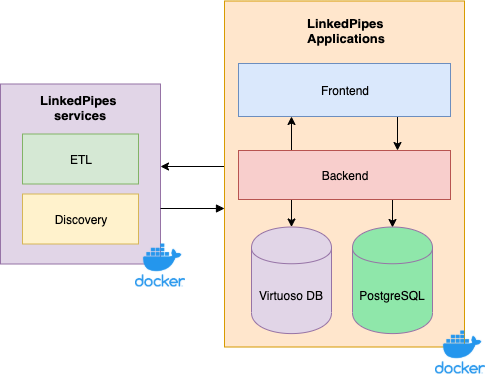
\includegraphics[width=12cm]{lpa_intro_architecture.png}
    \caption{High-level overview of \lpa{} platform}
    \label{fig:lpa_intro_architecture}
\end{figure}

Generally, we can categorize it into three main parts: 

\begin{itemize}
    \item \textbf{\lpa{}} - the main platform from LinkedPipes bundle that defines the functional and non-functional requirements for for \lpas{} project. Combines multiple database solutions for LinkedData, conventional SQL for storing user related records and implementation of a backend and frontend for creating applications.
    \item \textbf{LinkedPipes Services} - a set of external services provided from LinkedPipes bundle that \lpa{} heavily utilizes. Provides a toolset for identifying how linked data can be discovered, extracted, transformed and loaded into an RDF file for further processing.
\end{itemize}

\subsubsection{Frontend}

As mentioned at the beginning of the chapter, the frontend provides a way for the user to interact with the \lpa{}. The Redux \footnote{\url{https://redux.js.org}} and React \footnote{\url{https://reactjs.org}} are the leading technologies to be used during implementation. The main terms related to \lpa{} frontend that are commonly reffered to in \autoref{chap:num_4} and \autoref{chap:num_5} are described as follows:

\begin{itemize}
    \item \textbf{React Component} - a JavaScript class or function that optionally accepts inputs, i.e., properties(props), and returns a React element that describes how a section of the UI (User Interface) should appear. 
    \item \textbf{Redux} - represents a container that stores various states of the web application per individual webpage.
    	\subitem \textbf{State} - refers to the single state value that is managed by the store and returned by getState(). It represents the entire state of a Redux application, which is often a deeply nested object.
        \subitem \textbf{Reducer} - specifies how the application's state changes in response to actions sent to the store.
        \subitem \textbf{Actions} - are payloads of information that send data from your application to your store. They are the only source of information for the store. You send them to the store using store.dispatch().
        \subitem \textbf{Selector} - is simply any function that accepts the Redux store state (or part of the state) as an argument, and returns data that is based on that state.
\end{itemize}

Additionally, the \lpa{} frontend is the main component that is going to be improved by \lpas{}. This is due to specifics of a \solid{} toolset where most of the open-source libraries are implemented in JavaScript and are intended for usage in web based projects.

\subsubsection{Backend}

The function of the backend component is to provide a RESTful API that is used by the frontend component to execute user-requested actions and can also be used by other developers to create their user applications. The backend then implements the communication protocols with external services from LinkedPipes Services bundle. 

\subsubsection{PostgreSQL} 

The \lpa{} platform is storing all information related to users of the platform in an instance of a PostgreSQL database \footnote{\url{https://www.postgresql.org}}. 

PostgreSQL, often Postgres, is an object-relational database management system (ORDBMS) with an emphasis on extensibility and standards compliance. It can handle workloads ranging from small single-machine applications to large Internet-facing applications with many concurrent users.

The entities stored in the database are described as follows:
\begin{itemize}
\item User accounts.
\item Running instances of LinkedPipes discovery processes. The LinkedPipes Discovery component is described in detail \autoref{ssssec:linkedpipes_services}.
\item Running LinkedPipes ETL pipelines. The LinkedPipes ETL component is described in detail in \autoref{ssssec:linkedpipes_services}.
\item Custom templates of data sources generated by users.
\end{itemize}.

\subsubsection{Virtuoso DB}

Aside from PostgreSQL, another important database technology is OpenLink Virtuoso\footnote{\url{https://virtuoso.openlinksw.com}} which is used for storing all Linked Data sources processed by LinkedPipes ETL pipelines, and that is later used by \lpa{} visualizers. The important note to mention is that in contrast with PostgreSQL that is only used for all user-related information that needs to be stored, Virtuoso is only used for storing Linked Data. 

In general, Virtuoso Universal Server is a middleware and database engine hybrid that combines the functionality of a traditional Relational database management system (RDBMS), Object-relational database (ORDBMS), virtual database, RDF, XML, free-text, web application server and file server functionality in a single system. Rather than having dedicated servers for each of the functionality mentioned above, Virtuoso serves as a universal server instance.

\subsection{LinkedPipes Services} 
\label{ssssec:linkedpipes_services}

The LinkedPipes Services bundle demonstrated on \autoref{fig:lpa_intro_architecture} consists of two open-source software solutions developed under the Faculty of Mathematics and Physics at Charles University in Prague. They serve as the providers of core Linked Data processing functionality for \lpa{} platform. Since a significant technical knowledge in Semantic Web is required to use the tools independently, the \lpa{} platform provides a layer on top of them to simplify interactions with those components and make it available for any generic \textit{lay} user. 

\subsubsection{ETL} 

LinkedPipes ETL is an RDF-based, lightweight \gls{ETL} tool for Linked Data (\cite{klimek2016linkedpipes_etl}). It is not only a stand-alone application, but it also exposes a \acrshort{API} through which third-parties can execute the ETL process. 

\subsubsection{Discovery} 

LinkedPipes Discovery is a service used by \lpa{} platform to discover whether provided LinkedData sources can be processed and visualized by the platform. After a successful request sent to the Discovery service, it executes a session called \textit{Discovery session}. Upon successful completion of a Discovery session, service generates specific files in JSON-LD format. Those files are called \textit{pipelines}. A pipeline describes how LinkedPipes ETL needs to extract the whole LinkedData set and store the data into a Virtuoso database, which is a component used by the LinkedPipes Applications platform described earlier. 